% -------------------------------------------------------------------------
\subsection{Point forecasting and horizon decomposition}
\label{app:point}

Table~\ref{tab:point} gives the complete point comparison retained for
continuity with the intermittent-demand literature. Rankings exclude the
deliberately degenerate Zero and Naive-last rows. \REMIX{} takes six of
ten MAE/RMSSE cells and is top two on seven, but the result is not uniform:
classical methods retain several point-metric wins, and Zero attains the
lowest MAE on Online Retail, Carparts, and RAF. This is why the main text
uses point accuracy as a secondary diagnostic.

\begin{table*}[t]
\centering
\caption{Point forecasting across the five panels (lower is better;
bold best and underline second among non-degenerate methods). Degenerate
rows are shown as metric diagnostics and excluded from ranking.}
\label{tab:point}
\small
\setlength{\tabcolsep}{3.4pt}
\begin{tabular}{lcc@{\hspace{10pt}}cc@{\hspace{10pt}}cc@{\hspace{10pt}}cc@{\hspace{10pt}}cc}
\toprule
 & \multicolumn{2}{c}{Online Retail} & \multicolumn{2}{c}{M5} & \multicolumn{2}{c}{Auto} & \multicolumn{2}{c}{Carparts} & \multicolumn{2}{c}{RAF}\\
\cmidrule(lr){2-3}\cmidrule(lr){4-5}\cmidrule(lr){6-7}\cmidrule(lr){8-9}\cmidrule(lr){10-11}
Model & MAE & RMSSE & MAE & RMSSE & MAE & RMSSE & MAE & RMSSE & MAE & RMSSE\\
\midrule
CrostonClassic & 6.3294 & 5.1051 & 1.2345 & 2.3539 & 3.4056 & 1.1488 & 0.6792 & 1.0981 & 2.7315 & 1.6280\\
CrostonSBA & 6.1953 & 5.0692 & 1.2076 & 2.3517 & \secondbest{3.3325} & \secondbest{1.1451} & 0.6628 & 1.0935 & 2.6520 & 1.6272\\
TSB & \secondbest{5.5736} & 4.8031 & 1.2672 & 2.3612 & 3.6587 & 1.2066 & \best{0.5396} & 1.0156 & \best{2.1660} & 1.6570\\
TSB-tuned & 5.6318 & 4.7985 & \best{1.1932} & \secondbest{2.3137} & 3.3917 & 1.1452 & \best{0.5396} & 1.0156 & \secondbest{2.2447} & 1.6408\\
ADIDA & 5.6860 & \secondbest{4.7967} & 1.2274 & 2.3398 & 3.4079 & 1.1545 & 0.5556 & 1.0244 & 2.2977 & \secondbest{1.6245}\\
IMAPA & 5.7000 & 4.7970 & 1.2317 & 2.3280 & 3.4143 & 1.1555 & \secondbest{0.5524} & 1.0126 & 2.2850 & 1.6259\\
AutoARIMA & 6.5494 & 4.8175 & 1.2283 & 2.3169 & 3.4417 & 1.1745 & 0.5822 & \secondbest{1.0105} & 2.3153 & 1.6262\\
AutoTheta & 8.2862 & 4.8550 & 1.2988 & 2.3143 & 3.7490 & 1.2215 & 0.5704 & \best{0.9966} & 2.3687 & 1.6399\\
\midrule
Zero & 4.7549 & 4.8089 & 1.2995 & 2.4629 & 4.1444 & 1.4454 & 0.3867 & 1.0949 & 1.1717 & 1.6345\\
Naive-last & 6.0570 & 4.8324 & 1.3750 & 2.5450 & 4.3529 & 1.3818 & 0.5399 & 1.1408 & 1.8340 & 1.7644\\
\midrule
\REMIX{} (ours) & \best{5.5325} & \best{4.7901} & \secondbest{1.2032} & \best{2.2938} & \best{3.2145} & \best{1.1374} & 0.5726 & 1.0120 & 2.3874 & \best{1.6245}\\
\bottomrule
\end{tabular}
\end{table*}

\begin{figure}[t]
\centering
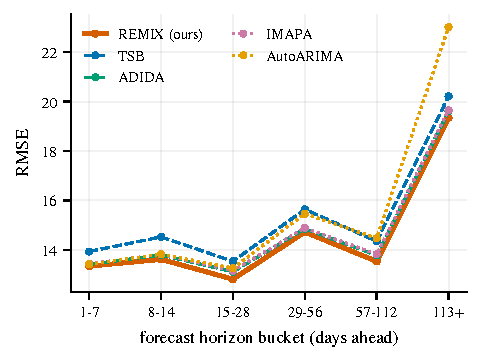
\includegraphics[width=0.93\linewidth]{figs/horizon_decomp.pdf}
\caption{Online Retail RMSE by fixed-origin forecast-horizon bucket.
\REMIX{} is lowest in every bucket, so the aggregate result is not
created by averaging only over distant horizons. MAE differences among
the leading methods are within $1$--$2\%$ by bucket.}
\label{fig:horizon}
\end{figure}

The selected $(g,w)$ pairs are: Online Retail (global, $0.95$), M5
(mixture, $0.95$), Auto (global, $0.99$), Carparts (global, $0.90$), and
RAF (mixture, $0.997$). On three of the five panels the margins between
pooling structures on the internal validation surface are under a tenth
of a percent, so the structure component of these pairs should be read as
Section~\ref{sec:leverage} reads it: the selector avoids poor structural
corners, and no winner is announced where the surface does not resolve
one.

\subsection{Selector diagnostics}
\label{sec:selector-diagnostics}
\label{app:selector-diagnostics}

The selection surface is locally flat near its optimum: on Online Retail
the best seven candidates span all three pooling structures and lie within
$0.51\%$ of one another in validation SPL. Section~\ref{sec:leverage}
reports the credibility leverage and refinement gains that accompany each
selected pair, and Figure~\ref{fig:refinement-leverage} places them
against the controlled panels. The selector is useful for choosing a
discount and for avoiding poor structural corners; the winning pooling
structure on a panel whose candidates lie within a tenth of a percent
should not be read as a scientific taxonomy. Per-panel selection surfaces
are released with the code.

\begin{table*}[t]
\centering
\caption{Full Online Retail ablation corresponding to
Table~\ref{tab:ablation}. Each row is an independent run; ``auto'' denotes
its own internal discount selection. TSB has no native predictive
distribution. Lower is better.}
\label{tab:ablation-full}
\small
\setlength{\tabcolsep}{5.0pt}
\begin{tabular}{llrrrrrr}
\toprule
Pooling & Forget & MAE & RMSE & RMSSE & SPL & SPL$_{90}$ & AIW\\
\midrule
none (TSB) & fixed & 5.5736 & 18.7272 & 4.8031 & --- & --- & ---\\
global & off & 5.7623 & \best{17.6892} & \best{4.7851} & 0.8899 & 1.5306 & 10.51\\
taxonomy & off & 5.7663 & \secondbest{17.6930} & \secondbest{4.7875} & 0.8897 & 1.5299 & 10.56\\
learned & off & 5.8126 & 17.7064 & 4.7876 & 0.8905 & 1.5336 & 10.79\\
global & auto ($.95$) & \best{5.5325} & 17.8386 & 4.7901 & \secondbest{0.8849} & \secondbest{1.5268} & \best{9.25}\\
taxonomy & auto ($.95$) & \secondbest{5.5624} & 17.8421 & 4.7897 & \best{0.8846} & \best{1.5254} & 9.43\\
learned & auto ($.95$) & 5.6925 & 17.8765 & 4.7902 & 0.8869 & 1.5343 & 10.69\\
\bottomrule
\end{tabular}
\end{table*}

\subsection{Walk-forward point results and protocol}
\label{app:walkforward}

\begin{table}[t]
\centering
\caption{Online Retail point forecasting under strict seven-day
walk-forward updates. The hierarchical rows differ in their
initialization discount and pooling structure.}
\label{tab:walkforward}
\small
\setlength{\tabcolsep}{5pt}
\begin{tabular}{lccc}
\toprule
Model & MAE & RMSE & RMSSE\\
\midrule
CrostonClassic & 5.692 & 16.937 & 4.854\\
CrostonSBA & 5.586 & 16.931 & 4.836\\
TSB & 5.434 & 17.754 & 4.815\\
ADIDA & \best{5.320} & \best{16.728} & \secondbest{4.637}\\
IMAPA & \secondbest{5.332} & \secondbest{16.745} & \best{4.632}\\
AutoARIMA & 5.482 & 16.904 & 5.105\\
AutoTheta & 5.394 & 16.836 & 4.735\\
\midrule
Stationary hierarchy ($w=1$) & 5.586 & 17.260 & 4.725\\
Forgetting hierarchy (tax., $.95$) & 5.411 & 17.059 & 4.682\\
\REMIX{} (selected global, $.95$) & 5.421 & 17.188 & 4.696\\
\bottomrule
\end{tabular}
\end{table}

\begin{table*}[t]
\centering
\caption{Full Online Retail probabilistic walk-forward results. SPL is
reported at all five quantiles and on average; Cov@80 is marginal
coverage and Cov$^{+}$@80 conditions on positive demand. CP and ACI
wrappers refit each block; AutoARIMA, AutoTheta, and iETS refit every four
blocks; \REMIX{} updates sufficient statistics each block.}
\label{tab:wfprob-full}
\small
\setlength{\tabcolsep}{4.2pt}
\begin{tabular}{lrrrrrrrr}
\toprule
Model & q10 & q25 & q50 & q75 & q90 & Mean & Cov@80 & Cov$^{+}$@80\\
\midrule
CP-Croston & 0.341 & 0.778 & 1.364 & 1.745 & 2.632 & 1.372 & 0.793 & 0.479\\
CP-SBA & 0.334 & 0.762 & 1.343 & 1.725 & 2.722 & 1.377 & 0.793 & 0.482\\
CP-TSB & 0.451 & 0.899 & 1.289 & 1.385 & 2.842 & 1.373 & 0.795 & 0.468\\
CP-ADIDA & 0.277 & 0.627 & 1.050 & \secondbest{1.319} & 2.514 & 1.158 & 0.791 & 0.473\\
CP-IMAPA & 0.292 & 0.660 & 1.084 & 1.329 & 2.522 & 1.177 & 0.791 & 0.471\\
AutoARIMA & 0.259 & 0.572 & 1.197 & 1.763 & 1.522 & 1.063 & 0.933 & 0.762\\
AutoTheta & 0.232 & 0.584 & 1.276 & 1.717 & \secondbest{1.483} & 1.059 & 0.931 & 0.765\\
iETS & 0.236 & 0.505 & 1.302 & 1.562 & 1.940 & 1.109 & 0.598 & 0.166\\
ACI-ADIDA & \secondbest{0.186} & \secondbest{0.468} & \best{0.909} & 1.324 & 1.668 & \secondbest{0.911} & 0.904 & 0.646\\
ACI-TSB & 0.189 & 0.482 & 0.948 & 1.384 & 1.709 & 0.942 & 0.904 & 0.641\\
Zero (diagnostic) & 0.183 & 0.458 & 0.916 & 1.374 & 1.649 & 0.916 & 0.740 & 0.000\\
\midrule
\REMIX{} & \best{0.183} & \best{0.458} & \secondbest{0.910} & \best{1.319} & \best{1.400} & \best{0.854} & 0.901 & 0.621\\
\bottomrule
\end{tabular}
\end{table*}

\begin{table*}[t]
\centering
\caption{Full Carparts monthly walk-forward SPL. Every statistical
baseline refits each block; \REMIX{} updates sufficient statistics.
The zero row is excluded from ranking.}
\label{tab:wf-carparts-full}
\small
\setlength{\tabcolsep}{5pt}
\begin{tabular}{lrrrrrr}
\toprule
Model & q10 & q25 & q50 & q75 & q90 & Mean\\
\midrule
AutoARIMA & 0.151 & 0.282 & 0.537 & 0.644 & 0.484 & 0.419\\
AutoTheta & 0.120 & 0.253 & 0.523 & 0.658 & \secondbest{0.474} & 0.406\\
CP-TSB & 0.141 & 0.301 & 0.487 & \secondbest{0.513} & 0.476 & 0.384\\
CP-ADIDA & \secondbest{0.096} & \secondbest{0.230} & \secondbest{0.411} & 0.529 & 0.488 & 0.351\\
CP-IMAPA & 0.101 & 0.235 & 0.413 & 0.518 & 0.479 & \secondbest{0.349}\\
iETS & 0.272 & 0.368 & 0.493 & 0.532 & 0.515 & 0.436\\
Zero (diagnostic) & 0.075 & 0.187 & 0.374 & 0.560 & 0.672 & 0.374\\
\midrule
\REMIX{} & \best{0.075} & \best{0.187} & \best{0.372} & \best{0.481} & \best{0.458} & \best{0.315}\\
\bottomrule
\end{tabular}
\end{table*}

\REMIX{} applies the selected discount once to the initialization
sufficient statistics and then accumulates revealed blocks without
compounding it. On Online Retail, ACI-ADIDA improves the static conformal
wrapper substantially and wins q50 by a hair, but \REMIX{} takes every
other quantile, the mean, and q90 by a clear margin. On Carparts the
first two quantiles saturate at zero and the discriminating gains occur
from the median up. Re-running joint selection at every block is not
evaluated.

\subsection{Significance and interval diagnostics}
\label{sec:significance}

\begin{table}[t]
\centering
\caption{Per-series mean SPL paired tests: \REMIX{} versus every
comparator on each panel, Holm-adjusted within panel (paired $t$ and
Wilcoxon signed-rank; the family includes TweedieGP on the monthly
panels). Cells count comparators by outcome at the $5\%$ level; named
entries are the comparators for which \REMIX{} is \emph{not}
significantly better.}
\label{tab:spl-significance}
\small
\setlength{\tabcolsep}{4.0pt}
\begin{tabular}{lcccl}
\toprule
Panel & Family & Sig.\ better & Sig.\ worse & Undecided\\
\midrule
Online Retail & 9 & 9 & 0 & ---\\
M5 & 9 & 5 & 0 & CP wrappers (4)\\
Auto & 10 & 10 & 0 & ---\\
Carparts & 10 & 9 & 0 & TweedieGP\\
RAF & 10 & 10 & 0 & ---\\
\bottomrule
\end{tabular}
\end{table}

\begin{table}[t]
\centering
\caption{Paired per-series MAE tests on Online Retail: \REMIX{} versus
each alternative. Negative mean differences favor \REMIX{}; $p$-values
are Holm-adjusted.}
\label{tab:significance}
\small
\setlength{\tabcolsep}{5pt}
\begin{tabular}{lccc}
\toprule
vs. & Mean diff & $p_t$ & $p_{\mathrm{Wilcoxon}}$\\
\midrule
Stationary hierarchy & $-0.165$ & $<10^{-29}$ & $<10^{-11}$\\
TSB & $-0.040$ & $0.532$ & $<10^{-155}$\\
TSB-tuned & $-0.090$ & $0.086$ & $<10^{-72}$\\
ADIDA & $-0.036$ & $0.359$ & $<10^{-88}$\\
IMAPA & $-0.049$ & $0.281$ & $<10^{-97}$\\
CrostonSBA & $-0.872$ & $<10^{-26}$ & $<10^{-59}$\\
AutoARIMA & $-0.891$ & $<10^{-14}$ & $<10^{-12}$\\
AutoTheta & $-2.644$ & $<10^{-81}$ & $<10^{-104}$\\
\bottomrule
\end{tabular}
\end{table}

\begin{table}[t]
\centering
\caption{Raw \REMIX{} interval quality across panels at nominal $80\%$
coverage. No post-hoc calibration is used.}
\label{tab:coverage}
\small
\setlength{\tabcolsep}{4.6pt}
\begin{tabular}{lccccc}
\toprule
 & OR & M5 & Auto & Carparts & RAF\\
\midrule
Coverage@80 & 0.892 & 0.846 & 0.907 & 0.931 & 0.921\\
AIW@80 & 9.25 & 2.81 & 9.21 & 1.47 & 0.94\\
\bottomrule
\end{tabular}
\end{table}

Table~\ref{tab:spl-significance} tests the headline metric directly:
per-series mean SPL, \REMIX{} against every comparator of
Table~\ref{tab:prob}, with paired $t$ and Wilcoxon signed-rank tests
Holm-adjusted within each panel and a comparison counted as decided only
when both adjusted tests agree at the $5\%$ level. \REMIX{} is
significantly better in 43 of the 48 panel--comparator pairs and
significantly worse in none. The five undecided pairs are informative
rather than embarrassing: on M5 the mean difference favors \REMIX{}
against all four conformal wrappers but the paired $t$ does not reach
significance after correction (the Wilcoxon strongly rejects symmetry,
so the per-series differences are systematic but heavy-tailed), and on
Carparts neither \REMIX{} nor TweedieGP separates from the other
(adjusted $p\ge0.50$ both ways), consistent with the half-percent
aggregate margin between them.

The paired MAE tests support a systematic improvement over the stationary
hierarchy. Against TSB, tuned TSB, ADIDA, and IMAPA, mean MAE favors
\REMIX{} but the adjusted paired $t$-tests are not significant; the
Wilcoxon tests reverse because those methods win on the typical series
while \REMIX{} reduces the difficult-series tail. On per-series RMSE,
both adjusted tests favor \REMIX{} against every comparator at $p<0.05$.
Raw intervals mildly over-cover, most strongly on Carparts.

\begin{figure}[t]
\centering
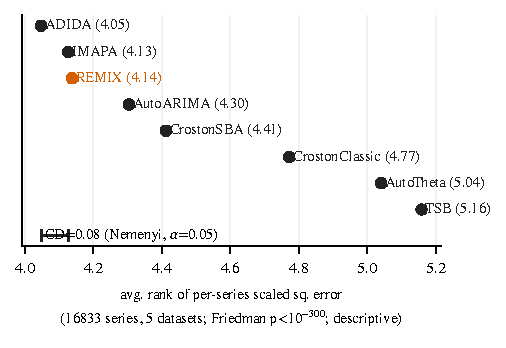
\includegraphics[width=0.93\linewidth]{figs/cd_diagram.pdf}
\caption{Average ranks of per-series scaled squared errors over the
16{,}833 series with complete saved row-level point predictions across
the five panels. The critical-difference bar is shown only for scale:
series, rather than datasets, are the blocks, so this is descriptive and
not a valid Friedman--Nemenyi test.}
\label{fig:cd}
\end{figure}

\subsection{Selection objective and efficiency}
\label{sec:criterion}\label{sec:efficiency}

The selector is not mathematically tied to pinball loss; it scores the
criterion supplied on the chronological validation tail. We use
item-averaged SPL because the target is a predictive distribution. The
best candidates are locally close, and a full cross-objective regret
matrix remains future work.

Joint selection takes $51$--$243$ seconds across the five panels,
excluding data loading, and covers 24 forecast candidates with one
deterministic EM/BIC search for the mixture on the fitting head. Final
estimation is analytic apart from low-dimensional group optimization;
selection and point prediction are deterministic, while probabilistic
bootstrap averaging uses the released fixed seed.

\subsection{Controlled-study diagnostics}
\label{app:simulation-details}

In the length sweep used to isolate credibility leverage, the generator
holds $K=2$, 500 items per group, occurrence probabilities $0.05$ and
$0.80$, log-size centers three units apart, and $w=1$. The true
partition's pinball advantage falls monotonically from $1.53\%$ at
$T=12$ (median 4.5 positives per item) to $0.01\%$ at $T=400$ (median
154), with NLL, Brier, and log-size MSE following the same direction.
Across the main grid, the RMSE of $\hat\tau_g^2$ approximately doubles
as $w$ falls from $1.00$ to $0.90$ ($0.037\to0.144$ at $T=120$ and
$0.074\to0.149$ at $T=30$), directly measuring the resolution cost in
Proposition~\ref{prop:twosided}.

The generator centers the groups symmetrically around a fixed grand mean
so that increasing separation does not change total demand scale, and
every arm is evaluated through the same hurdle-lognormal predictive
representation under both likelihood-based proper scores and point
metrics. A four-arm ladder---single pool, true labels with estimated
hyperparameters, true labels with true hyperparameters, and the true
conditional law---checks the implementation; the true conditional law is
best on every metric in every cell.
